% ------------------------------------------------------------------------
% ------------------------------------------------------------------------
% abnTeX2: Modelo de Trabalho Academico (tese de doutorado, dissertacao de
% mestrado e trabalhos monograficos em geral) em conformidade com 
% ABNT NBR 14724:2011: Informacao e documentacao - Trabalhos academicos -
% Apresentacao
% ------------------------------------------------------------------------
% ------------------------------------------------------------------------

\documentclass[
	% -- opções da classe memoir --
	12pt,				% tamanho da fonte
	openright,			% capítulos começam em pág ímpar (insere página vazia caso preciso)
	%twoside,			% para impressão em verso e anverso. Oposto a oneside
	oneside,
	a4paper,			% tamanho do papel. 
	% -- opções da classe abntex2 --
	%chapter=TITLE,		% títulos de capítulos convertidos em letras maiúsculas
	%section=TITLE,		% títulos de seções convertidos em letras maiúsculas
	%subsection=TITLE,	% títulos de subseções convertidos em letras maiúsculas
	%subsubsection=TITLE,% títulos de subsubseções convertidos em letras maiúsculas
	% -- opções do pacote babel --
	english,			% idioma adicional para hifenização
	french,				% idioma adicional para hifenização
	spanish,			% idioma adicional para hifenização
	brazil				% o último idioma é o principal do documento
	]{abntex2}

% ---
% Pacotes básicos 
% ---
\usepackage{lmodern}			% Usa a fonte Latin Modern			
\usepackage[T1]{fontenc}		% Selecao de codigos de fonte.
\usepackage[utf8]{inputenc}		% Codificacao do documento (conversão automática dos acentos)
\usepackage{lastpage}			% Usado pela Ficha catalográfica
\usepackage{indentfirst}		% Indenta o primeiro parágrafo de cada seção.
\usepackage{color}				% Controle das cores
\usepackage{graphicx}			% Inclusão de gráficos
\usepackage{microtype} 			% para melhorias de justificação
\usepackage[font={small,it}]{caption}
% ---
		
% ---
% Pacotes adicionais, usados apenas no âmbito do Modelo Canônico do abnteX2
% ---
\usepackage{lipsum}				% para geração de dummy text
% ---

% ---
% Pacotes de citações
% ---
\usepackage[brazilian,hyperpageref]{backref}	 % Paginas com as citações na bibl
\usepackage[alf]{abntex2cite}	% Citações padrão ABNT

% define o caminho das imagens
\graphicspath{{Imagens/}}

% --- 
% CONFIGURAÇÕES DE PACOTES
% --- 

% ---
% Configurações do pacote backref
% Usado sem a opção hyperpageref de backref
\renewcommand{\backrefpagesname}{Citado na(s) página(s):~}
% Texto padrão antes do número das páginas
\renewcommand{\backref}{}
% Define os textos da citação
\renewcommand*{\backrefalt}[4]{
	\ifcase #1 %
		Nenhuma citação no texto.%
	\or
		Citado na página #2.%
	\else
		Citado #1 vezes nas páginas #2.%
	\fi}%
% ---

% ---
% Informações de dados para CAPA e FOLHA DE ROSTO
% ---
\titulo{Título Provisório da Monografia de\\ Trabalho de Conclusão de Curso}
\autor{Rodrigo Mendonça da Paixão \\ Lucas Teles Agostinho}
\local{São Paulo -- Brasil}
\data{2015}
\orientador{Eduardo Heredia}
%\coorientador{Nome Completo}
\instituicao{%
  Centro Universitário Senac
  \par
  Bacharelado em Ciência da Computação
}
\tipotrabalho{Monografia (Graduação)}
% O preambulo deve conter o tipo do trabalho, o objetivo, 
% o nome da instituição e a área de concentração 
\preambulo{Pré-monografia apresentada na disciplina Trabalho de Conclusão de Curso I, como parte dos requisitos para obtenção do título de Bacharel em Ciência da Computação.}
% ---

% ---
% Configurações de aparência do PDF final

% alterando o aspecto da cor azul
\definecolor{blue}{RGB}{41,5,195}

% informações do PDF
\makeatletter
\hypersetup{
     	%pagebackref=true,
		pdftitle={\@title}, 
		pdfauthor={\@author},
    	pdfsubject={\imprimirpreambulo},
	    pdfcreator={LaTeX with abnTeX2},
		pdfkeywords={abnt}{latex}{abntex}{abntex2}{trabalho acadêmico}, 
		colorlinks=true,       		% false: boxed links; true: colored links
    	linkcolor=blue,          	% color of internal links
    	citecolor=blue,        		% color of links to bibliography
    	filecolor=magenta,      		% color of file links
		urlcolor=blue,
		bookmarksdepth=4
}
\makeatother
% --- 

% --- 
% Espaçamentos entre linhas e parágrafos 
% --- 

% O tamanho do parágrafo é dado por:
\setlength{\parindent}{1.3cm}

% Controle do espaçamento entre um parágrafo e outro:
\setlength{\parskip}{0.2cm}  % tente também \onelineskip

% ---
% compila o indice
% ---
\makeindex
% ---

% ----
% Início do documento
% ----
\begin{document}

% Retira espaço extra obsoleto entre as frases.
\frenchspacing 

% ----------------------------------------------------------
% ELEMENTOS PRÉ-TEXTUAIS
% ----------------------------------------------------------
% \pretextual

% ---
% Capa
% ---
\imprimircapa
% ---

% ---
% Folha de rosto
% (o * indica que haverá a ficha bibliográfica)
% ---
\imprimirfolhaderosto%*
% ---

% ---
% RESUMOS
% ---

% resumo em português
\setlength{\absparsep}{18pt} % ajusta o espaçamento dos parágrafos do resumo
\begin{resumo}
   
 \textbf{Palavras-chaves}: IDS,Rede,Internet
\end{resumo}

% ---
% inserir lista de ilustrações (figuras)
% ---
\pdfbookmark[0]{\listfigurename}{lof}
\listoffigures*
\cleardoublepage
% ---

% ---
% inserir lista de tabelas
% ---
\pdfbookmark[0]{\listtablename}{lot}
\listoftables*
\cleardoublepage
% ---

% ---
% inserir lista de abreviaturas e siglas
% ---
\begin{siglas}
  \item[IDS] Intrusion Detection System
  \item[IPS] Intrusion Prevention System
  \item[NIDS] Network Intrusion Detection System
  \item[IA] Inteligência Artificial
  \item[RNA] Rede Neural Artificial
  \item[AG] Algotitimo genético
\end{siglas}
% ---

% ---
% inserir o sumario
% ---
\pdfbookmark[0]{\contentsname}{toc}
\tableofcontents*
\cleardoublepage
% ---

% ----------------------------------------------------------
% ELEMENTOS TEXTUAIS 
% ----------------------------------------------------------
\textual

% ----------------------------------------------------------
% Capitulo 1
% ----------------------------------------------------------
\chapter[Introdução]{Introdução}
%\addcontentsline{toc}{chapter}{Introdução}
% ----------------------------------------------------------

\section{Contexto}

Analisar e melhorar os sistemas de detecção de intrusao é uma abordagem importante nos dias atuais, aonde a segurança da informação é essencial, torna-se necessario analisar formas de detectar tentativas de lesar a integridade, confidencialidade ou disponibilidade desta.

O trabalho dos sistemas de detecção de intrusão (IDS) é monitorar as atividades e analisar os eventos em um rede em busca de anomalias que sugiram uma invasão.Estes não costumam executar qualquer ação para impedir intrusões, sua principal função é alertar os administradores de sistemas que há uma possível violação de segurança, sendo assim uma ferramenta pró-ativa em vez de reativa[3].

Podemos classifar os IDS da seguinte forma. 

Baseado em Host ou baseado em rede aonde o primeiro faz uso de arquivos de log de cada computador individualmente e o segundo captura pacotes que trafegam na rede para analisar seu conteudo.

Online ou Offline, onde um é capaz de detectar e marcar um instruso enquanto a esta sendo realizida a intrusão, e o outro analisa registros após o evento ocorrer e indica que houve uma violação de segurança tinha ocorrido desde a última verificação, respectivamente.

Baseado em abuso ou baseado em anomalia, onde por anomalia o sistema identifica comportamento fora do padrão, e por abuso compara as atividades na rede com comportamentos de ataques já conhecidos.

Muitos dos metodos utilizados nos IDS são baseados em inteligencia artificial, tais como Algoritimo genetico(AG)[4] e Redes Neurais Artificiais (RNA)[2][5].

Algoritmo genético é uma família de modelos computacionais baseados em princípios de evolução e seleção natural. Esses algoritmos convertem o problema de um domínio específico para um modelo usando uma estrutura de dados  \"cromossomo" de forma a evoluir estes cromossomos usando operadores de seleção, recombinação e mutação[4]. 
O processo de um algoritmo genético geralmente começa com uma população selecionada aleatoriamente de cromossomos. estes cromossomos são representações do problema a ser resolvido. De acordo com os atributos do problema, diferentes posições de cada cromossomo são codificados como bits, caracteres ou números. Estas posições são muitas vezes referidos como genes e são alterados aleatoriamente dentro de um intervalo durante a evolução. 

As RNA são uma classe de algoritimos para aprendizado de maquina, usada para realizar classificação de dados. A rede neural é treinada de forma a dar mais importancia para as principais caracteristicas de uma determinada instancia de um problema, para ajudar a classificar os dados que ainda estão por vir. 
RNAs tem sido utilizadas com sucesso na detecção de intrusão [6][7][8],no entanto ela necessita de uma quantidade substanciao de dados para tralizar o trinamento antes de receber os dados novos para classificação, por causa dessa limitação elas nao são capazes de serem bem treinadas em casos de baixa frequencia de ataques, resultando em uma baixa taxa de acerto na detecção[9]


\section{Motivação}

Apesar de vários esforços de prover a segurança em redes, o número,variedade e complexidade dos incidentes relacionados à segurança tem crescido(Figura 1)[1].

\begin{figure}[!htb]
     \centering
     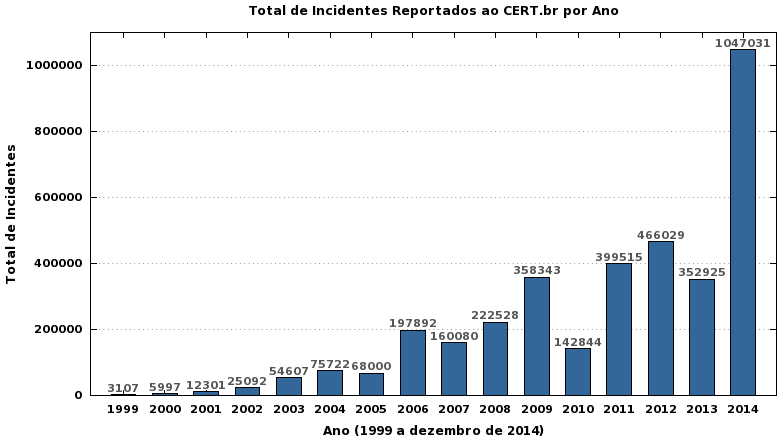
\includegraphics[scale=0.5]{Imagens/IntroGraf.png}
     \caption{Incidentes ano a ano. Fonte: (CERT/CC, 2015)}
\end{figure}

Com isso é necessario pensar em abordagens mais sofisticadas para IDS, como utilização de abordagens hibridas diferentes relativo a tecnicas de IA, estas já têm sido exploradas para ultrapassar os problemas de qualquer um dos métodos individuais[10][11][12]. 


\section{Objetivos}
Temos como objetivo criar uma ferramenta que seja de fácil uso e posso ser usada por outros desenvolvedores em suas aplicações, onde irá detectar um ou mais tipos de ataques conhecidos e alguns semelhantes,dando um baixo número de erros.

\section{Método de trabalho}



\section{Organização do trabalho}



% ----------------------------------------------------------
% Capitulo 2
% ----------------------------------------------------------
\chapter[Revisão de Literatura]{Revisão de Literatura}
%\addcontentsline{toc}{chapter}{Revisão de Literatura}
% ----------------------------------------------------------
\section{Segurança e Detecção de intrusão}

O IDS usa padrões ja conhecidos de atividades ilegais para indentificar se o comportamento esta diferente do perfil tradicional, porém não é incomun ocorrer os chamados falsos negativos ou falsos positivos, isso ocorre por existir uma margem de erro nestas classificações. 
Após isso para negar o serviço ao intruso é necessario o uso de um Sistema de Prevenção de Intrusão (Intrusion Prevention System - IPS), este é uma solução ativa que provê políticas e regras para o tráfego de rede, quanto o IDS somente avisa a atividade suspeita, o IPS tenta parar essa atividade, porém também possui uma taxa de erro.
Com a popularização de ferramentas e técnicas cada vez mais sofisticadas de intrusão é necessario criar ferramentas e tecnicas mais sofisticadas para IDS e IPS.

O objetivo é criar um sistema de detecção de intrução que apresente um baixo indice de erros utilizando tecnicas de inteligencia artificial, onde o sistema vai aprender, quais são os comportamentos aceitos na rede de computadores.

Os principais objetivos da segurança computacional são:

\textbf{Confidencialidade}: a garantia de que a informação esteja disponível somente para aqueles que tem autorização para obtê-la.

\textbf{Integridade}: é a garantia de que a informação permanecerá inalterada mesmo sob situações críticas, como acidentes ou tentativas de manipulações hostis.

\textbf{Disponibilidade}: consiste na proteção dos recursos e serviços prestados pelo sistema de forma que eles não sejam degradados ou se tornem indisponíveis garantindo assim que a informação estará sempre acessível e pronta para o uso.



Qualquer atividade que possa comprometer qualquer um desses
objetivos é considerada uma violação às políticas de segurança.

 \section{Ameaças à segurança}

 As falhas de segurança são contantes nos sistemas computacionais, essas os sujeitam a varios tipos de ameaças internas ou esternas, que podem acabar desencadeando intrusoes que exploram as vulnerabilidades do sistema.  

 A motivação para exploração dessas vulnerabilidades podem ser de simples vandalismo até tecnicas de espionagem.

Segundo um relatório técnico gerado pelo Sandia National Laboratories (HOWARD; LONGSTAFF, 1998) é apresentado uma taxonomia que se baseia em ações para classificar ameaças à segurança em cima das informações que estão em transito. 

As caracteristicas destas são (podem ser visualizadas na figura 2):

\textbf{Interrupção:} As informações em trânsito são interrompidas, impossibilitando que as mesmas cheguem até seu destino e prejudicando a questão da disponibilidade dos recursos.

\textbf{Interceptação:} As informações são interceptadas durante a transmissão, comprometendo a confidencialidade da mensagem.

\textbf{Modificação:} As informações são interceptadas e alteradas 
durante a transmissão, afetando não só a confidencialidade como a integridade da mensagem.

\textbf{Fabricação:} Trata-se da inserção de informações em determinada comunicação, comprometendo a autenticidade das informações recebidas.

\begin{figure}[!htb]
     \centering
     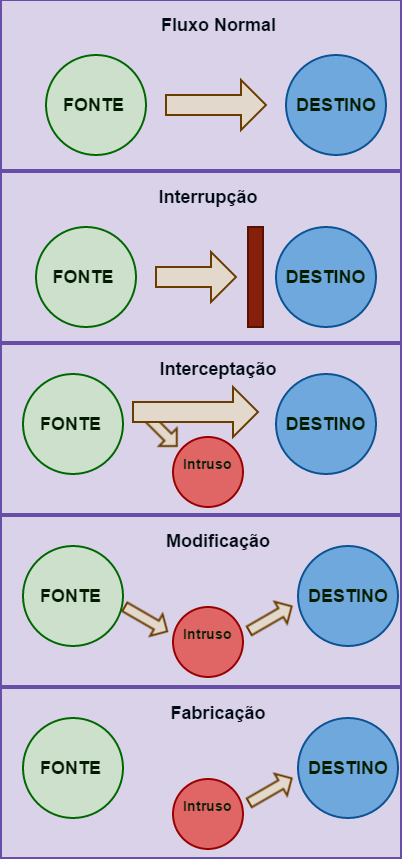
\includegraphics[scale=0.8]{Imagens/Classificacoes.png}
     \caption{Taxonomia baseada em ações}
\end{figure}


% ----------------------------------------------------------
% Capitulo 3
% ----------------------------------------------------------
\chapter[Proposta do Trabalho]{Proposta do Trabalho (O que vai ser desenvolvido!)}
%\addcontentsline{toc}{chapter}{Metodologia}
% ----------------------------------------------------------


% ----------------------------------------------------------
% Capitulo 4
% ----------------------------------------------------------
\chapter[Expectativas]{Expectativas}
%\addcontentsline{toc}{chapter}{Expectativas}
% ---



% ----------------------------------------------------------
% ELEMENTOS PÓS-TEXTUAIS
% ----------------------------------------------------------
\postextual
% ----------------------------------------------------------

% ----------------------------------------------------------
% Referências bibliográficas
% ----------------------------------------------------------
\chapter[Bibliografia]{Bibliografia}
\bibliography{abntex2-modelo-references}
%\bibliography{bib/monografia.bib}
[1] CERT/CC. CERT/CC Statistics 1988-2015. Computer Emergency Response
Team (Coordenation Center), Maio 2015. Acessado em 22/05/2015. Disponível
em: <http://www.cert.br/stats/>.

[2] Shraddha Surana, “Intrusion Detection using Fuzzy Clustering and Artificial Neural Network” Research Scholar, Department of Computer Engineering, Vishwakarma Institute of Technology, Pune, 2014

[3] W. W. Fu and L. Cai, “A Neural Network based Intrusion Detection Data Fusion Model,” in Third International Joint Conference on Computational Science and Optimization, 2010. 

[4] Wei Li, Using Genetic Algorithm for Network Intrusion Detection, Department of Computer Scienceand Engineering Mississippi State University, Mississi ppi State, MS 39762 

[5] Jake Ryan, Meng-Jang Lin and Risto Miikkulainen. Intrusion Detection with Neural
Networks. In Advances in Neural Information Processing Systems 10, MIT Press, 1998.


[6] C. Zhang, J. Jiang and M. Kamel, “Intrusion
Detection using hierarchical neural
networks,” Pattern Recognition Letters, pp.
779-791, 2005.

[7] X. Tong, Z. Wang and H. Yu, “A research
using hybrid RBF/ Elman neural networks for
intrusion detection system secure model,”
Computer Physics Communication, pp. 1795-
1801, 2009.

[8] S.-C. O. K. Y. Wonil Kim, “Intrusion
Detection Based on Feature Transform Using
Neural Network,” in Computational Science -
ICCS 2004, vol. 3037, Springer Berlin
Heidelberg, 2004, pp. 212-219

[9] R. Beghdad, “Critical study of neural networks in detecting intrusions,” Computers \& Security, pp. 168-175, 2008.

[10] G. Liu, Z. Yi and S. Yang, “A hierarchical
intrusion detection model based on the PCA
neural networks,” Neurocomputing, pp. 1561-
1568, 2007.

[11] L. Ren, “Research of Web Data Mining based
on Fuzzy Logic and Neural Networks,” in
Sixth International Conference on Fuzzy
Systems and Knowledge Discovery, 2006.

[12] F. M.-P. F. J. M.-G. R. L.-F. J. A. G.-M.-A.
D. M.-J. Iren Lorenzo-Fonseca, “Intrusion
detection method using Neural Networks
based on the reduction of characteristics,” in
Bio-Inspired Systems: Computational and
Ambient Intelligence, vol. 5517, Springer
Berlin Heidelberg, 2009, pp. 1296-1303.


\end{document}
